
\documentclass{article}

\title{A New Solution to Hydrogen}
\author{Brent Baccala}
\date{February 8, 2023}

\usepackage{amsmath}

\usepackage{xcolor}
\usepackage{comment}
\usepackage{graphicx}

\usepackage[hidelinks]{hyperref}

\usepackage{tabularx}

\begin{document}
\parindent 0pt

\maketitle

\begin{abstract}
I show a previously unknown exact solution to the simplest time-independent Schr\"odinger equation for hydrogen.
The solution involves a Bessel function, is not separable, and is not in $L^2$.
\end{abstract}

\subsection*{Theorem}

Consider the following simple Sch\"odinger equation for the hydrogen atom:

\begin{equation}
\label{schrodinger}
-\frac{1}{2}\nabla^2 \Psi - \frac{1}{r}\Psi = E \Psi
\end{equation}

Let $J_0$ be the ordinary Bessel function $J_0$, and set

\begin{equation}
\label{solution}
\Psi = J_0(2\sqrt{x+r})
\end{equation}

where $x,y,z$ are Cartesian coordinates and $r=\sqrt{x^2+y^2+z^2}$.

\vskip 12pt

Then \eqref{solution} is an exact solution to \eqref{schrodinger}, with $E=0$.

\subsection*{Verification}

The result can be easily verified using Mathematica, as follows:

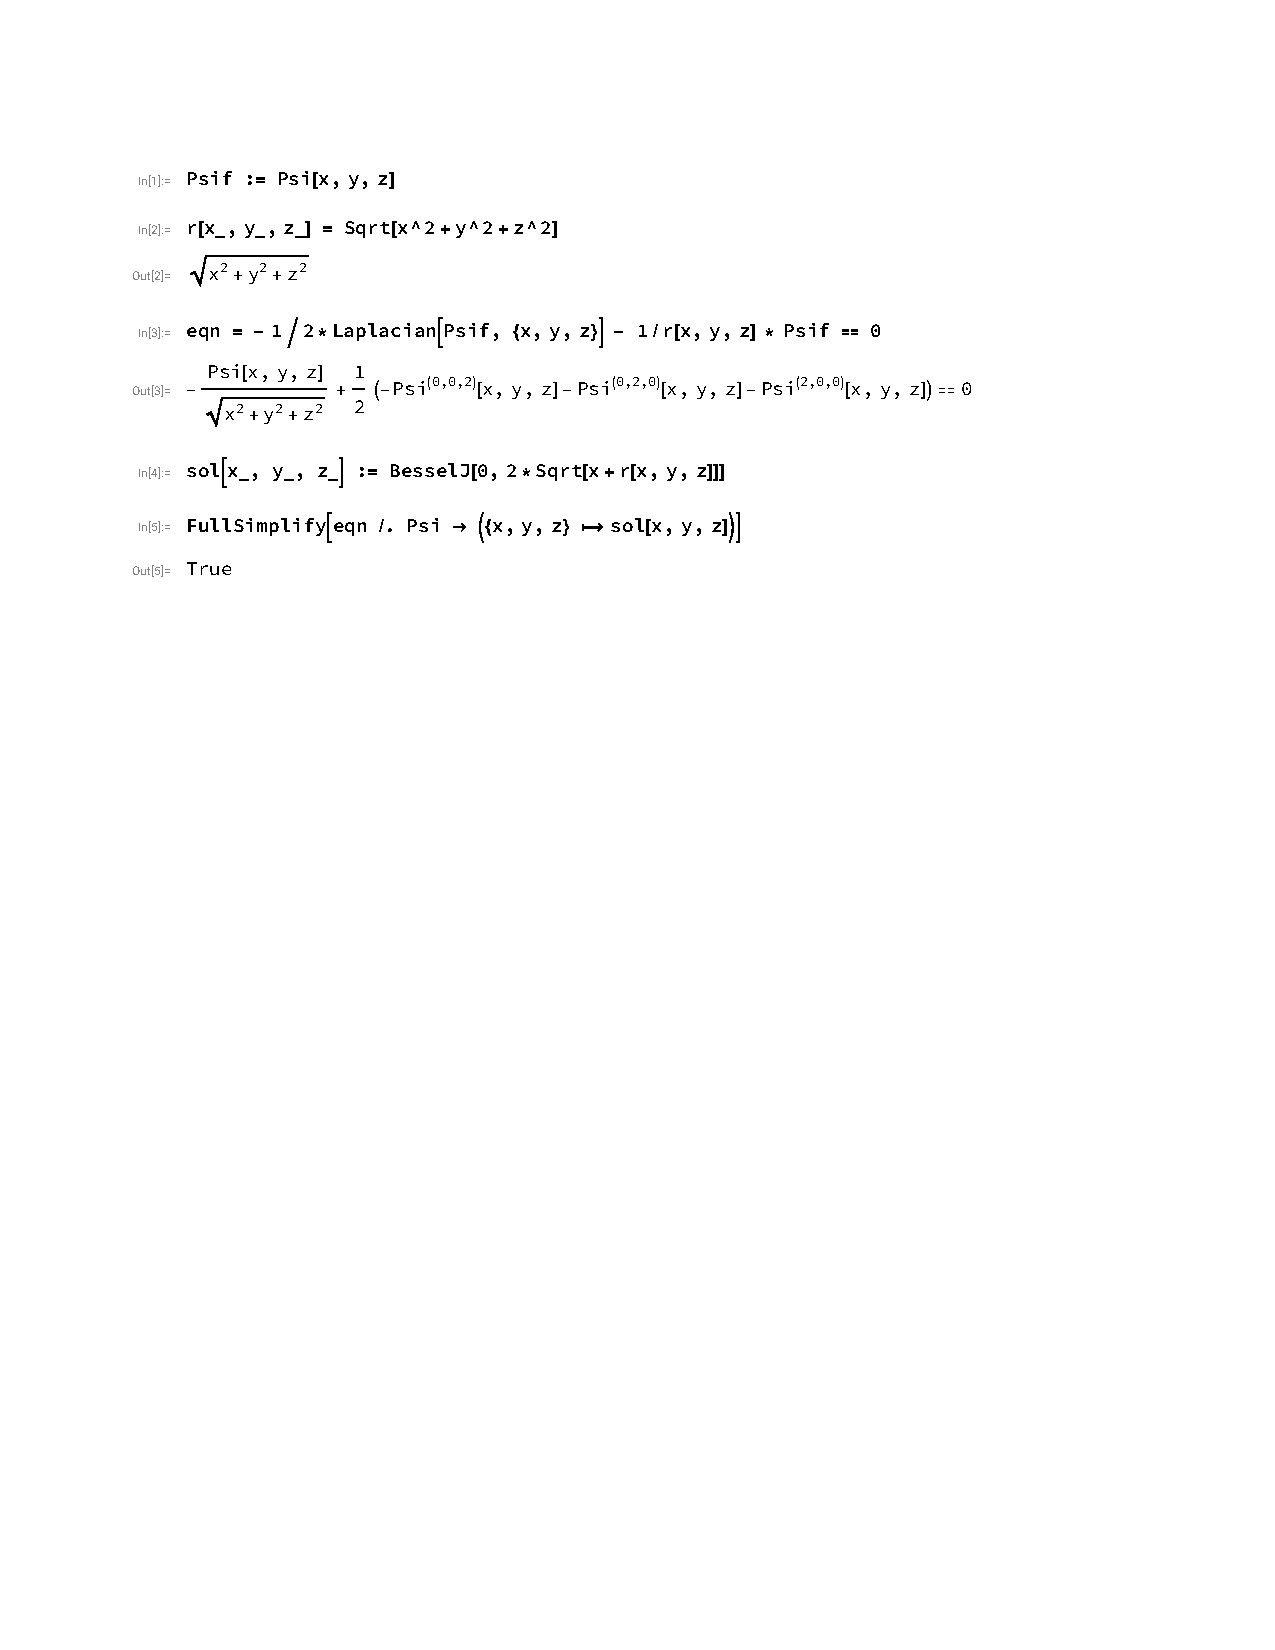
\includegraphics[page=1, clip, trim=1in 7in 1in 1in, width=\textwidth]{improved.pdf}

\vfill\eject
\subsection*{Proof}
The claim is that $\Psi = J_0(2\sqrt{x+r}) = (J_0 \circ 2\sqrt{v}) (x+r)$ satisfies:

\begin{equation}
\label{claim}
\left(\frac{\delta^2}{\delta^2 x} + \frac{\delta^2}{\delta^2 y} + \frac{\delta^2}{\delta^2 z}\right) \Psi + \frac{2}{r}\Psi = 0
\end{equation}

Letting $v=x+r$, we compute the first partial derivatives of $\Psi$:

%\begin{equation}
%\frac{\delta}{\delta x} \Psi = \frac{d v}{d x} \frac{d}{d v}  \Psi = \frac{d v}{d x} J_0'(v) x^{-1/2}
%\end{equation}

\begin{subequations}
\begin{align}
\frac{\delta \Psi}{\delta x} = \frac{d v}{d x} \frac{d}{d v} \left(J_0 \circ 2\sqrt{v}\right) = \frac{d v}{d x} J_0'(2\sqrt{v}) v^{-1/2} \\
\frac{\delta \Psi}{\delta y} = \frac{d v}{d y} \frac{d}{d v} \left(J_0 \circ 2\sqrt{v}\right) = \frac{d v}{d y} J_0'(2\sqrt{v}) v^{-1/2} \\
\frac{\delta \Psi}{\delta z} = \frac{d v}{d z} \frac{d}{d v} \left(J_0 \circ 2\sqrt{v}\right) = \frac{d v}{d z} J_0'(2\sqrt{v}) v^{-1/2}
\end{align}
\end{subequations}

Next we compute the partial second derivatives of $\Psi$:

\begin{subequations}
\label{second partials}
\begin{align}
\frac{\delta^2 \Psi}{\delta x^2} = \frac{d^2 v}{d x^2} J_0'(2\sqrt{v}) v^{-1/2} + \left(\frac{d v}{d x}\right)^2 J_0''(2\sqrt{v}) v^{-1} - \frac{1}{2} \left(\frac{d v}{d x}\right)^2 J_0'(2\sqrt{v}) v^{-3/2} \\
\frac{\delta^2 \Psi}{\delta y^2} = \frac{d^2 v}{d y^2} J_0'(2\sqrt{v}) v^{-1/2} + \left(\frac{d v}{d y}\right)^2 J_0''(2\sqrt{v}) v^{-1} - \frac{1}{2} \left(\frac{d v}{d y}\right)^2 J_0'(2\sqrt{v}) v^{-3/2} \\
\frac{\delta^2 \Psi}{\delta z^2} = \frac{d^2 v}{d z^2} J_0'(2\sqrt{v}) v^{-1/2} + \left(\frac{d v}{d z}\right)^2 J_0''(2\sqrt{v}) v^{-1} - \frac{1}{2} \left(\frac{d v}{d z}\right)^2 J_0'(2\sqrt{v}) v^{-3/2}
\end{align}
\end{subequations}

We need to know the derivatives of $v=r+x$ with respect to the coordinates:

\begin{subequations}
\label{first v}
\begin{align}
\frac{d v}{d x} = & \frac{d}{d x} (x+r) = 1 + \frac{x}{r} \\
\frac{d v}{d y} = & \frac{d}{d y} (x+r) = \frac{y}{r} \\
\frac{d v}{d z} = & \frac{d}{d z} (x+r) = \frac{z}{r}
\end{align}
\end{subequations}

\begin{subequations}
\label{second v}
\begin{align}
\frac{d^2 v}{d x^2} = \frac{d}{d x} \left(1 + \frac{x}{r}\right) = & \frac{r - x(x/r)}{r^2} = \frac{r^2 - x^2}{r^3} \\
\frac{d^2 v}{d y^2} = & \frac{r^2 - y^2}{r^3} \\
\frac{d^2 v}{d z^2} = & \frac{r^2 - z^2}{r^3}
\end{align}
\end{subequations}

\vskip 20pt

Substituting \eqref{first v} and \eqref{second v} into \eqref{second partials}, and \eqref{second partials}
into the LHS of \eqref{claim}, we obtain:

\begin{equation*}
\begin{aligned}
&\frac{d^2 v}{d x^2} J_0'(2\sqrt{v}) v^{-1/2} + \left(\frac{d v}{d x}\right)^2 J_0''(2\sqrt{v}) v^{-1} - \frac{1}{2} \left(\frac{d v}{d x}\right)^2 J_0'(2\sqrt{v}) v^{-3/2} \\
+& \frac{d^2 v}{d y^2} J_0'(2\sqrt{v}) v^{-1/2} + \left(\frac{d v}{d y}\right)^2 J_0''(2\sqrt{v}) v^{-1} - \frac{1}{2} \left(\frac{d v}{d y}\right)^2 J_0'(2\sqrt{v}) v^{-3/2} \\
+& \frac{d^2 v}{d z^2} J_0'(2\sqrt{v}) v^{-1/2} + \left(\frac{d v}{d z}\right)^2 J_0''(2\sqrt{v}) v^{-1} - \frac{1}{2} \left(\frac{d v}{d z}\right)^2 J_0'(2\sqrt{v}) v^{-3/2} \\
+& \frac{2}{r} J_0(2\sqrt{v})
\end{aligned}
\end{equation*}

\begin{equation*}
\begin{aligned}
=&\frac{r^2-x^2}{r^3} J_0'(2\sqrt{v}) v^{-1/2} + (1+\frac{x}{r})^2 J_0''(2\sqrt{v}) v^{-1} - \frac{1}{2} (1+\frac{x}{r})^2 J_0'(2\sqrt{v}) v^{-3/2} \\
&+ \frac{r^2-y^2}{r^3} J_0'(2\sqrt{v}) v^{-1/2} + \left(\frac{y}{r}\right)^2 J_0''(2\sqrt{v}) v^{-1} - \frac{1}{2} \left(\frac{y}{r}\right)^2 J_0'(2\sqrt{v}) v^{-3/2} \\
&+ \frac{r^2-z^2}{r^3} J_0'(2\sqrt{v}) v^{-1/2} + \left(\frac{z}{r}\right)^2 J_0''(2\sqrt{v}) v^{-1} - \frac{1}{2} \left(\frac{z}{r}\right)^2 J_0'(2\sqrt{v}) v^{-3/2} \\
&+ \frac{2}{r} J_0(2\sqrt{v})
\end{aligned}
\end{equation*}

\begin{equation*}
\begin{aligned}
=&\frac{3r^2-x^2-y^2-z^2}{r^3} J_0'(2\sqrt{v}) v^{-1/2} + (1+2\frac{x}{r} +\frac{x^2}{r^2} + \frac{y^2}{r^2} + \frac{z^2}{r^2}) J_0''(2\sqrt{v}) v^{-1} \\
&- \frac{1}{2} (1+2\frac{x}{r} +\frac{x^2}{r^2}+ \frac{y^2}{r^2} + \frac{z^2}{r^2}) J_0'(2\sqrt{v}) v^{-3/2} \\
&+ \frac{2}{r} J_0(2\sqrt{v})
\end{aligned}
\end{equation*}

\begin{equation*}
=\frac{2}{r} J_0'(2\sqrt{v}) v^{-1/2} + (2+2\frac{x}{r}) J_0''(2\sqrt{v}) v^{-1} - \frac{1}{2} (2+2\frac{x}{r}) J_0'(2\sqrt{v}) v^{-3/2} + \frac{2}{r} J_0(2\sqrt{v})
\end{equation*}

\begin{equation*}
=\frac{2}{r} J_0'(2\sqrt{v}) v^{-1/2} + (2+2\frac{x}{r}) J_0''(2\sqrt{v}) v^{-1} - \frac{x+r}{r} J_0'(2\sqrt{v}) v^{-3/2}
+ \frac{2}{r} J_0(2\sqrt{v})
\end{equation*}

Remembering that $v=x+r$,

\begin{equation*}
=\frac{2}{r} J_0'(2\sqrt{v}) v^{-1/2} + (2+2\frac{x}{r}) J_0''(2\sqrt{v}) v^{-1} - \frac{1}{r} J_0'(2\sqrt{v}) v^{-1/2}
+ \frac{2}{r} J_0(2\sqrt{v})
\end{equation*}

\begin{equation*}
=\frac{2}{r} J_0'(2\sqrt{v}) v^{-1/2} + \frac{2}{r} J_0''(2\sqrt{v}) - \frac{1}{r} J_0'(2\sqrt{v}) v^{-1/2}
+ \frac{2}{r} J_0(2\sqrt{v})
\end{equation*}

\begin{equation*}
=\frac{2}{r} J_0''(2\sqrt{v}) + \frac{1}{r} J_0'(2\sqrt{v}) v^{-1/2} + \frac{2}{r} J_0(2\sqrt{v})
\end{equation*}

\begin{equation*}
=\frac{2}{r} J_0''(2\sqrt{v}) + \frac{2}{r\cdot2\sqrt{v}} J_0'(2\sqrt{v}) + \frac{2}{r} J_0(2\sqrt{v})
\end{equation*}

\begin{equation}
\label{last eq in derivation}
=\frac{2}{r} \left( J_0''(2\sqrt{v}) + \frac{1}{2\sqrt{v}} J_0'(2\sqrt{v}) + J_0(2\sqrt{v})\right)
\end{equation}

Now, the ordinary Bessel function $J_0(x)$ satisfies:

\begin{equation*}
x^2 J_0''(x) + xJ_0'(x) + x^2J_0(x) = 0
\end{equation*}

dividing through by $x^2$ and changing variables, we get:

\begin{equation*}
J_0''(2\sqrt{v}) + \frac{1}{2\sqrt{v}}J_0'(2\sqrt{v}) + J_0(2\sqrt{v}) = 0
\end{equation*}

which shows that \eqref{last eq in derivation} is zero, and establishes the proof of \eqref{claim}.

\subsection*{Generalization}

The choice of $x$ is arbitrary, and any ordinary Bessel function can be used:

\begin{equation}
\label{generalized solution}
\Psi = F(2\sqrt{a_1 x+ a_2 y+ a_3 z+r})
\end{equation}

where

\begin{equation*}
a_1^2+a_2^2+a_3^2=1
\end{equation*}

and $F$ is any linear combination of the Bessel functions $J_0$ and $Y_0$.

\vskip 12pt

Any finite linear combination of functions of the form \eqref{generalized solution} also solves \eqref{schrodinger}.

\subsection*{Contact}

The author maintains a discussion page for this result on his personal blog at:

\begin{center}
\small
\url{https://www.freesoft.org/blogs/soapbox/a-new-solution-to-hydrogen/}
\end{center}

\end{document}
